\documentclass[a4paper,11pt]{article}

% \usepackage[lf]{Baskervaldx}       % text
% \usepackage[bigdelims,vvarbb]{newtxmath} % math
% \usepackage[cal=boondoxo]{mathalfa}      % \mathcal

% \usepackage[T1]{fontenc}
% \usepackage{baskervillef}                 % text

\usepackage{CormorantGaramond} % not bad too

% \usepackage[light]{antpolt} % not bad too
% \usepackage[T1]{fontenc}

\usepackage{gfsartemisia-euler}
\usepackage[T1]{fontenc}

% \usepackage{fontspec}
% \setmainfont{QTChanceryType} % cool font
% QTChanceryType % another cool font

% For nice fonts, check https://tug.org/FontCatalogue/seriffontscategorised.html

\usepackage[baskerville,vvarbb]{newtxmath} % math tuned for BaskervilleF
\usepackage[cal=boondoxo]{mathalfa}

\usepackage{microtype}
\usepackage{graphicx}
\graphicspath{{FIG/}}
\usepackage{amsmath} % don't load amssymb with unicode-math

\usepackage{color}
\usepackage[table]{xcolor}
\usepackage{eso-pic}
\usepackage{longtable}
\usepackage{sidecap}

\setlength{\fboxsep}{3pt}
\tolerance=1000000
\hyphenpenalty=5000
\setcounter{tocdepth}{2}

\definecolor{lightblue}{rgb}{.94,.94,1.}
\definecolor{lightgreen}{rgb}{1.,.94,.94}
\definecolor{green}{rgb}{.94,1.,.94}
\definecolor{bluemy2}{rgb}{0.,0.,0.4}
\definecolor{redmy2}{rgb}{0.7,0.1,0.}
\definecolor{gray1}{rgb}{0.4,0.4,0.4}
\definecolor{graybox}{rgb}{0.94,0.94,0.94}
\definecolor{refcolor}{rgb}{0.3,0.3,0.3}

\usepackage{hyperref}
\hypersetup{
  pdftitle={Human-led Science in the Age of Superintelligence},
  pdfauthor={Vladislav A. Yastrebov},
  pdfsubject={Superintelligence, Science},
  pdfcreator={LaTeX},
  pdfkeywords={Superintelligence, Science, Human Science, Purpose and meaning, Frontiers of knowledge},
  pdfnewwindow=true,
  colorlinks=true,
  linkcolor=refcolor,
  citecolor=refcolor,
  filecolor=refcolor,
  urlcolor=refcolor
}
\usepackage{cleveref}

\let\openbox\relax

\usepackage{amsthm}
\newtheorem{hypothesis}{Hypothesis}

% Optional: nicer refs
\usepackage{cleveref}
\crefname{hypothesis}{Hypothesis}{Hypotheses}



\newcommand{\ie}{\emph{i.e.\ }}
\newcommand{\eg}{\emph{e.g.\ }}
\newcommand{\etc}{\emph{etc.\ }}
\newcommand{\etal}{\emph{et al.\ }}

\usepackage{nomencl}
\makenomenclature

\usepackage{longtable}
\usepackage{array}
\usepackage{booktabs}


\newenvironment{nomenclatureO}{%
  \section*{Nomenclature}
  \setlength{\LTpre}{0pt}  % Remove space before table
  \setlength{\LTpost}{1em} % Add space after table
  \begin{longtable}{@{}p{2.5cm}p{11cm}@{}}
    \toprule
    \textbf{Abbreviation} & \textbf{Description} \\
    \midrule
    \endfirsthead
    
    \multicolumn{2}{@{}l}{\textit{Continued from previous page}} \\
    \toprule
    \textbf{Abbreviation} & \textbf{Description} \\
    \midrule
    \endhead
    
    \midrule
    \multicolumn{2}{@{}r}{\textit{Continued on next page}} \\
    \endfoot
    
    \bottomrule
    \endlastfoot
}{%
  \end{longtable}
}

\usepackage[backend=biber,style=authoryear,dashed=false]{biblatex}
\addbibresource{references.bib}
\DeclareDelimFormat{nameyeardelim}{\addcomma\space}

\title{Human-led Science in the Age of Superintelligence}
\author{Vladislav A. Yastrebov}
\date{\footnotesize\textit{Sant Cugat del Vall\`es, Spain}\\
\textit{Pamplona, Spain}\\
\textit{Moret-Loing-et-Orvanne, France}\\
August 2025}

\begin{document}

\maketitle

\thispagestyle{empty}
\begin{center}
    \includegraphics[width=1\textwidth]{Fig_SI_v2.jpg}
    \textit{A Thinker on the Mount Everest's Summit}\footnote{This figure refers to ``The Great Flood'' analogy of a flooded landscape of human competence~\parencite{moravec1988mind,moravec1998will} -- when some cognitive tasks are performed better by machines than humans, the ``mountain''-analogy of this domain is shown as flooded -- arts and sciences were shown as highest peaks in this analogy. The waxing crescent moon signifies a dawn of the human intellectual domination (well this interpretation of the crescent moon makes sense in the Northern hemisphere, and thus on the altitude of Mount Everest).}

    \vspace{0.5cm}
    \footnotesize 
    \textbf{100\% human created content.} 
\end{center}

    \newpage



\begin{center}
    $ $\\
    \vspace{4.5cm}
    
\includegraphics[width=0.4\textwidth]{ai_usage.pdf}\\[1em]
    \footnotesize 
    \textbf{100\% human created content.} 
\end{center}
\vspace{-1em}
\footnotesize \noindent
\begin{quote}
This essay was written without usage of any AI/ML tools. All ideas, writing, creation of figures, editing, spelling, translation and grammar check -- all was done by Vladislav A. Yastrebov with zero tolerance to AI usage. It was a deliberate choice of the author. This choice, however, affects to some extent the quality of the text as the author is not a native English speaker. On the other hand, the readers can be sure that the wording of this essay keeps genuinely author's voice and that the ideas and their explications were not adjusted or deformed by an AI.
    
\end{quote}

\newpage

 	\tableofcontents


    % \printnomenclature


\newpage

    \section{Introduction}

    \noindent Does it matter for you if 
\begin{itemize}
    \item a book or a poem,
    \item a movie or a theater play,
    \item a painting or a photography,
    \item a song or a concerto,
    \item a sculpture or a cathedral,
    \item a dance or its choreography
\end{itemize}
was performed/created/generated/constructed by AI and not by a human with his/her own history, her/his mastering and his/her ``soul''? Probably, most of us prefer human-created art. But what about scientific progress and its components?
Will it matter for you if AI proves a theorem, constructs an experiment equipment and conducts experiments, collects and analyzes data, draw conclusions and develops new models and refines theories? Like or not, in the age of Superintelligence (SI), it will take care of all these aspects of scientific progress~\parencite{moravec1998will,moravec1999rise}. It will construct new neutrino and gravitational wave detectors, new particle colliders, send new missions to the Sun, to the planets and small bodies of our Solar System and to the outer space, conduct large scale social and political experiments, study all historical archives and in parallel, of course, SI will advance all theoretical sciences and maybe will create new ones. What about us? What about humans in the loop and, in particular, what about human scientists?

In this essay, I will consider possible futures of scientific exploration and in particular the role of humans (or our derivatives) in this future. Will we be simply archivists or ``priests'' and ``priestess'' in a temple of SI-led Science (SIS)? Or maybe, we will have our contribution to make to this new Science and even push our own, Human-led Science (HS) based either on the legacy science or near the forefront of the SIS? Will be active players of the true scientific research or simply science-game players in our virtual personal universe? Are our current, evolution-provided cognitive capacities, which are tuned mainly for survival and efficient reproduction, enough or we need a sort of augmentation biological or silicon-based? Will we push the science being always accompanied by a SI mentor or will we be able to do something on our own? Will SI share with us the entirety of its knowledge or discoveries and, more generally, what will be the relationship between HS and SIS? Will SI eventually stop in its exploration being satisfied by the world model it constructs in its ``mind'' or the progress will continue forever? These questions will be addressed in this essay.

\subsection{Notions}

Notions: SI, HS - Human-led Science\footnote{Human-led Science: either legacy science of science advancement without use of superintelligence} and Superintelligence Science\footnote{Superintelligence-led Science: knowledge acquired and advanced by the SI, notably for the purpose of an accurate world model.} (SIS), subgoals and World's most accurate model.


    \section{Raw}

    Current technology is already great and can get us rapidly much further in scientific progress. The technology develops too fast to let most of scientists catch up with its development pace.

    In many scenarios, in the world of Superintelligence (SI), most of human activities transform into a game, the same gamification is expected for the science, one of the most serious and demanding humans occupations.
    
    It will be an utopian essay\footnote{Probably, for people not familiar with the concept of post-instrumental deep utopia from Bostrom, this text will see too far beyond their short-term imagination. So, I would invite them to take a look on the concepts and tools introduced in \textcite{DeepUtopia}.} in the spirit of~\parencite{DeepUtopia} and \parencite{LovingGrace}, but we shall not forget that getting to this utopian state with a friendly SI presents \textit{per se} a great challenge -- the most important and the last challenge that the humanity will face. However, the objective of this essay is to reflect on the state of science when this "great filter" has been overcame and the humanity has a well-aligned SI at its disposal \parencite{Yudkowsky2008,Yampolskiy2016,Yudkowsky2022}. Let's dream.

    Oracle type SI -- human scientists will ask intelligent question, accumulate knowledge, synthetize it and make progress in Science, but it seems that the AI\footnote{Artificial Intelligence in a general sense.} development has not selected this path of development and a path of superpowerful and agentic "souverain" type, introduced by \textcite{Bostrom2014}, will prevail.

    With an SI, it is clear that the mankind is practically excluded from the advancement of the forefront science in important domains -- those which a critical for constructing an accurate world model. Then, will such occupation as "scientist" disappear completely? Probably not, because in a "solved world" a search for meaning will be crucial thought largely simplified by the SI, and a science-related occupation seems very appealing for those who value intelligence.

    Why SI will take lead in the scientific research? As known from~\parencite{Bostrom2014,Tegmark2017}, any goal provided to an AI -- super optimizer -- induces sub-goals such as self-preservation, access to resources and construction of an accurate world model.
    Nevertheless, it does not mean that answering all questions that are interesting for us, are beneficial for constructing this world model. Therefore, scientific progress of the SI can ignore some unresolved questions asked by humans. Nevertheless, the SI could be managed to make progress in this directions if needed. Such class of scientific domains and questions we will denote as idle scientific questions/domains.


\textbf{Fractal granularity of scientific landscape and its boundary}

    The pavement of scientific knowledge, or more specifically the boundary between known and unknown, between the ``terra cognita'' and ``terra incognita'', can be seen to some extent as a fractal surface in the sense that at the macroscopic scale of global domains we have a general understanding, on the smaller scale of particular details, we have a more detailed understanding and on smaller, microscopic scales we can have very specific questions, which for example can yet remain unanswered. Formulation and solution of such questions can lead to the refinement of our understanding, development of new methods and experiments, and even lead to new important subquestions\footnote{``The purpose of
models is not to fit the data but to sharpen the questions'', Samuel Karlin} representing further scales in this fractal knowledge landscape and eventually to some relevant discoveries. These small scales are critical for the advancement of the science. This fractal boundary between the known and unknown is fuzzy on the bigger scale and becomes clear on the smaller scales of specific questions. So, the advancement of the boundary can be ensured by clarifying these smaller scales. And an SI can see clearly the voids on these smaller scales and fill them in thus resulting to the gradual progress of the forefront. For the gradual and steady progress of the science, the amplitude of oscillations (standard deviation of the small scales from the average boundary) between the known and unknown shall be small enough. So I guess the frontiers of the SI-led science (SIS) can be smoother than this of the human-led Science (HS).

\textbf{Separation of HS and SIS}

It is essential to separate the SI-led Science (SIS) and the Human-led Science (HS). In the current HS, of course, nobody has a fine-granular understanding of the fractal boundary between the known and unknown but some scientists have a relatively broad vision of the fuzzy macroscale frontier at least in their own and neighboring domains. Some scientists really work on the forefront of the global HS frontier, and some are simply pushing their own boundaries which are located in the vicinity of already known. If asked, SI will be able to bring scientists to the forefront or at least closer to the forefront of HS or SIS. Currently, the HS' frontier can be cristallized but of course it exists nowhere but in the global and cleaned up scientific literature. Therefore, individual scientific boundary and the global HS' even at the smaller scales can differ drastically. Now, we need to imagine that the SIS' boundary spanning all domains, at least those relevant to the world model construction, will further differ from the HS' boundary. Can the humanity assume that this new frontier belongs to them too? Probably not, since there's none of living or had lived human individuals who understood (in a broad sense of this verb) this new boundary or made progress from the HS' frontier to the SIS' one. Therefore, one of possible human's occupation will be pushing the HS' frontiers closer to the SIS' one.

Sharing of information between HS and SIS is not symmetric. If eventually, by chance, humans make progress beyond the SIS' frontier, the later can readily integrate this progress. The opposite is not possible, the SI can and will advance the science for its world map construction and will not necessarily share its progress with humans. To transmit information, there should be a receiver on the human's side. So, such a transmission could be done in special cases, like in Oracle Temple analogy (see \Cref{sec:oracle}), but probably a real-time reception will not be possible because of the limited intellectual and bandwidth of the receivers, even if they are augmented. So, for some discoveries, maybe a life-long training will be needed to understand at least approximately the contours of the discovery. On the other hand, people have to be interested in receiving this information, maybe some domains will seem of zero interest for humans and thus no information will be shared. 

Moreover, in some domains with a high risk of ``black balls'' -- potentially destructive technologies\footnote{See a ``vulnerable world hypothesis'' by \textcite{VulnerableWorldHypothesis}.}, SI will probably prefer not to share new knowledge, let's call such domains ``human forbidden scientific domains''. Probably, even the frontiers of such domains can be protected, and the SI won't let any human in this buffer zone. However, maybe existing level of science is already sufficient to invent a black-ball technology. In overall, SI strategy about black balls' scientific zones is not an easy philosophical question and probably our access or its lack will depend on the type of alignment. 

With these devastating black-ball technologies, the benevolent SI should be very careful and protective. One potential scenario of block is non-intrusive external distraction of scientists and engineers trying to penetrate into the black-ball zone and construct a technology. This distraction could take a form similar to one imagined in a science fiction novel ``Definitely Maybe''\footnote{The original title of this novel -- ``A Billion Years Before the End of the World'' -- is much more meaningful in the context of SI and black ball risks.} from brothers Strugatsky. There, an astrophysicist who was about to make a revolutionary discovery finds himself continuously distracted from his scientific work by such an improbable sequence of events that the scientist deduces that something intelligent (Homeostatic intelligent Universe) prevents him from continue his study\footnote{As it nicely stated in \href{https://en.wikipedia.org/wiki/Definitely_Maybe_(novel)}{Wikipedia} ``... the mysterious force is the Universe's reaction to mankind's scientific pursuit, which threatens to destroy the very fabric of the universe in some distant future.''}. Ultimately, he abandons this topic. In the age of SI, this distraction can be much softer or even invisible. In the worst case scenario, if external non-intrusive distraction does not work, it can intervene intrusively by rewiring the brain of the intruder. Alternatively, SI will let us in but will prevent constructing a black-ball technology to protect humanity and the Universe. On its side, SI with its SI strategic planning should foresee very remote consequences of major scientific discoveries but even with the power of SI, forecasting the behavior of a chaotic dynamic system for one billion years will be far beyond its capacity.

Apart from protecting us from ``black ball'' innovations, we could try to instill in the proto-SI the seeds of ethical innovation and research~\parencite{grinbaum2013responsible,grinbaum2024responsible} in addition to general moral incetives which will be further deepen and developed by SI itself.

% So, if the pace of progress, at least in purely theoretically domains is

\textbf{New Toolbox}

Are our mathematics and tools well adapted to pushing further the science frontiers and go well beyond to the existing understanding? At least, to the current generation of scientists it would remain the most mastered and thus perfect tool for this endeavour. But maybe, SI would be able to suggest different tools and even different mathematics for this pursuit. Our mathematics, notations and tools are made for humans. Probably, SI will operate completely different notions and objects and will push the SIS' frontier in such a way that it will be completely obscure to the HS and thus an adaptation and translation might be required.

\textbf{Scale of the SI and the Energy Efficiency}

Necessarily, SI will have a perfect representation of a human brain functionality. Our brain is slow and not optimized by evolution\footnote{I cannot not cite here~\textcite{Scott2014Moloch} ``evolution is a blind idiot alien god that optimizes for stupid things and has no concern with human value''.} for purely cognitive function, but it is quite energy efficient compared to the current comparable AI consumption, it also learns and generalizes very fast and if we eventually get to the age of SI, \emph{per se} is the ultimate proof of our brain efficiency. At the same time, I believe that human brain's cognitive function can be made even more energy efficient by removing all extra functionality unnecessary for the cognitive function. Therefore, SI will be able to reproduce human-level intelligence with let's say 1\% of its energy consumption and if implemented on silicon or any other faster, non-biological support which would be $\approx$10,000 times faster (chemical signals in our brain are very slow compared to electric circuits). So we get already $10^6$ in efficiency gain.
With only this optimization (without increasing the number of neurons and its connections which as the scaling hypothesis), we can get a factor of a million in terms of efficiency compared to an ordinary human. If you remove emotions and distractions add an access to solid databases, such an information processing entity will be already a prototype SI. If you scale by a factor of 1,000 in terms of "neurons/connections", then you get a total factor of one billion in terms of efficiency of cognitive function and you can easily call it SI which can further self-develop. Maybe, there could be a trade off between the depth / speed and energy efficiency for the objective function and further expansion in scale would penalize the cognitive function, but anyway this factor is already quite beyond our perception of SI. Maybe already with a factor of a billion beyond the human brain's capacity, such an SI will be optimal for operating in our Universe but of course all will depend on the its goals. This factor can be of course further increased.

\textbf{Human emotion}

Human emotion of achievement and exciting is very important for the scientific progress. This emotional boost is purely human and is not required for a machine to construct its world model and push SIS. But if humans want to be in the loop, this emotional side of the science can be artificially added and the sense of the lack of purpose in rediscovery of SIS can be removed in the "post-instrumental" world~\parencite{DeepUtopia}. A further boost can be added by human's augmentation, which would represent, I think, a common practice in the HS in the future. The level of this augmentation could be deliberately selected and adjusted. This augmentation in terms of cyborgization or biological enhancement can provide us with higher mental ability and also can provide us with tools enabling us to advance faster to the frontiers of SIS.

\subsection{Social/Community Aspect and its Emulation, personal universe.\label{subsection:personal-universe}}
The community and the societal aspect of science are very important. These aspects could however be mimicked to let people engaged in HS feel good and surrounded by like minds. Social networks could be adjusted for individual scientists to provide them with additional (external) motivation and inspiration. Some ego-promoting aspects can be deployed: people, whatever their contribution, can become Einsteins in their small individually-tuned social universes. If having a social network with emulated agents praising you is not enough, you can be emerged in our personal universe adjusted for your values and your objectives as suggested by~\textcite{Yampolskiy2019}. So you can operate in any epoch and in any scientific role: be a star of quantum mechanics in early 20th century or be a scientist in a space expedition to a new imaginary inhabited world in our galaxy, you can even appear in a completely new world with different physics laws and fundamental constants imagined by SI and discover this new world as a pioneer scientist without a priori knowledge of it. You can adjust your mind to be part you and part a scientist of your choice with his/her mindset too, you can choose to be Henri Poincaré and work on the 3-body problem or, e.g. Galileo Galilei and discover Jupiter moons with your handmade telescope. Of course, all the environment of these epochs could be adjusted according to your preferences. Or you can live a life of Magister Ludi from Hesse's ``The Glass Bead Game'' practicing a pure abstract mixture of art and science in a ``Ivory tower''. However, the question of keeping youself remains very relevant. If you want to keep yourself, you'll need to limit augmentation and mindset change. However, you could keep the option to return to the original settings but keeping or not memories after spending a period in one universe. It all can be implemented in a personal universe projected to your five senses if you decide to keep your brain in our physical world or it could all happen in a digital world with you uploaded mind. The second seems to be technically simpler and energetically more efficient.

In your personal universe, you don't necessary push the science and do not necessary advance to SIS but can be simply happy doing science and living a fulfilling life.

\paragraph{Evolution of individual scope.} 
Over the last century, scientists have been becoming more narrow experts in specific topics. With SI in the loop and augmentation, we can broaden our individual scientific scope and operate within a broader scientific domain,~\Cref{fig:scope}. It will provide them with a better vision of science in general and of the frontier.

\begin{figure}
    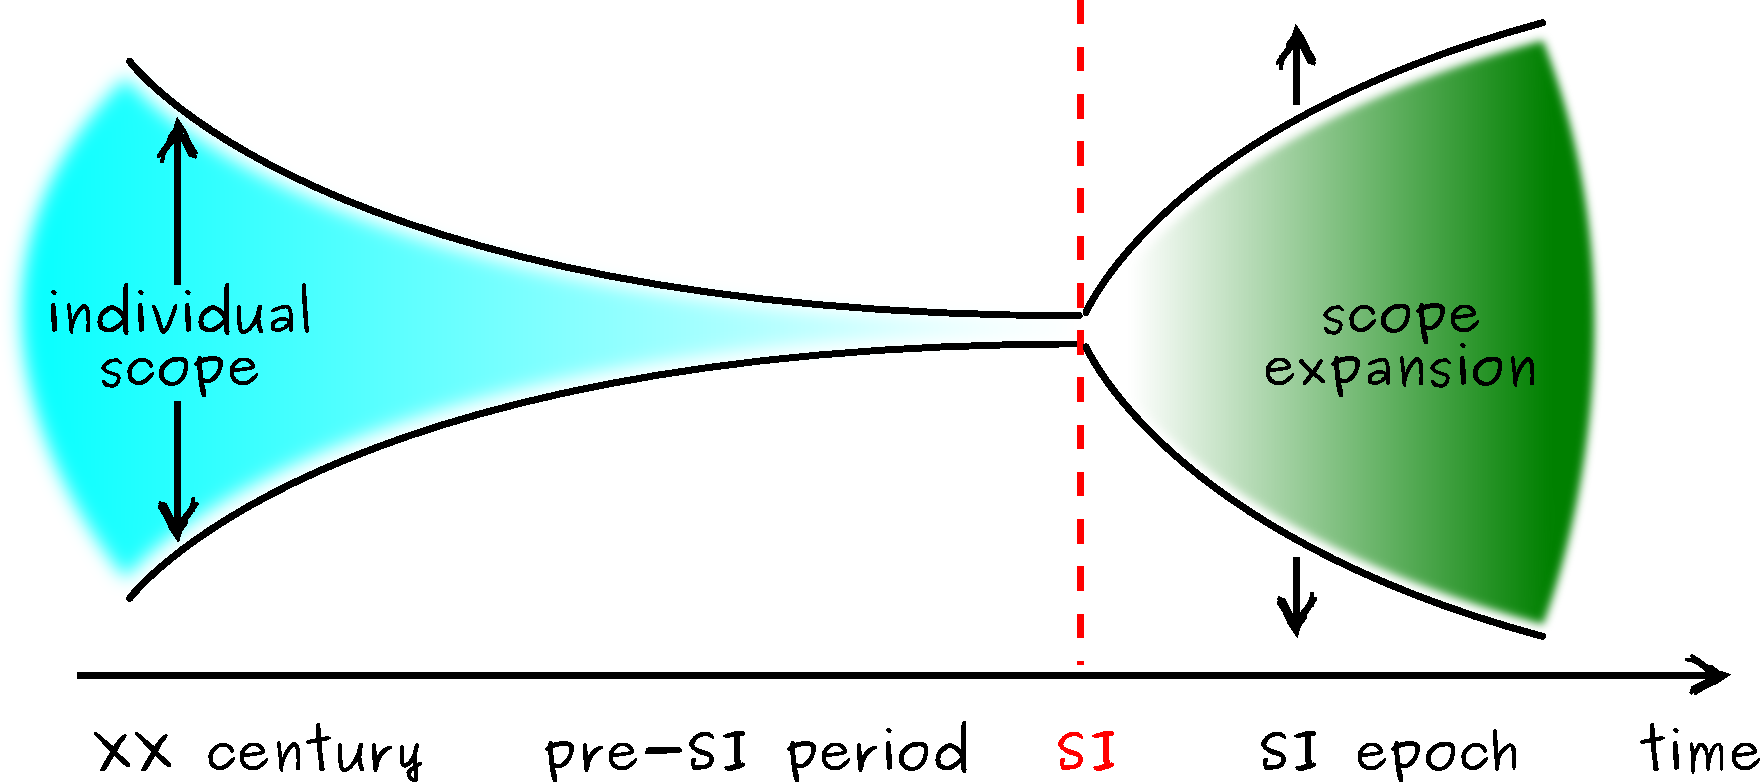
\includegraphics[width=1\textwidth]{scope}
    \caption{\label{fig:scope}Expansion of individual scientist's scientific scope in the SI epoch}
\end{figure}

\paragraph{Individual scale.}

At the individual scale, discovering new things makes a lot of sense even though it is not on the forefront of SIS nor even of HS. So if in any case the utilitarian function of HS will vanish in the solved world, the excitement part will remain there if, of course, humans decide to keep the current mind settings.

\paragraph{SI as a senior colleague and mentor.}

SI can help us to move forward towards the frontiers of SIS by motivating, encouraging and guiding. With such a wise mentor and colleague we will be able to focus only on relevant questions and limit our distractions, i.e. it will not let us exploring dead ends. So, our personal progress, being directed, will be more efficient\footnote{Instead of random walk advancing a distance proportional a square root of time $~\sqrt{t}$, we will be able to progress linearly $\sim t$ over the most efficient geodesic trajectory.}. However, the level of guidance can be adjusted, for example, instead of explicit guidance to the questions that matter, SI could give us hints that we could decipher: planets in a special arrangement, signs that we could notice during our morning rambling in a new city we are visiting, a quotation that we can occasionally read on a wall of a café where we drink our morning coffee. Of course, it all will be easier to implement in a digital universe.

When the questions of your scientific research are established and a path partially paved, SI can provide you with adapted reading, adjusted for your knowledge and brain's preferences in terms and in form, with probably some passages deliberately kept difficult, so it takes you some time to understand.
Or maybe you learn some new experimental techniques, tests them and finally deploy to understand some new (for you) in biology or particle physics.
So, you are encouraged to increase your mastering of the topic to pass some barriers and achieve the goal: prove a theorem, explore specific functions of some proteins or refine your understanding of strong interaction. Of course SI knows your current intellectual and work capacity, missing knowledge and your potential to make your own discovery and overcome the difficulty, so the problems can be perfectly adjusted and it can reveal to you that "you can do it". When we are sure that we can, then we truly can. It could be a finer message: "You can do it with 30\% probability." It would be more challenging but more rewarding. So, in such a set-up with a benevolent SI mentor, you can really surpass yourself and show the best of you. "I did believe that it was beyond your capacities, but you've finally proved this tricky theorem! Bravo!" - SI could deceive you with flattery in the end.

\paragraph{Science as a game/Playing in science.}

Humans have limited capacities in cognitive function, our speed is very limited as well as the number of tools we master and the broadness of topics we truly master. Even though we made tremendous progress in Science over the last couple of centuries, we won't be able to push the frontiers of science in the age of SI beyond the frontiers established by it. Nevertheless, we will be able ``to play'' in science. In any case it will be not about pushing science but if you wish it could be about believing\footnote{This could be done by adjustment of the brain or of its version uploaded into a simulation.} that you push it in an environment or entire universe crafted for you.

\paragraph{SI oracle and its priests\label{sec:oracle}}

Future scientist can serve as priests and priestess in a temple of SI oracle (analogous to a research center) by asking smart questions and documenting the answers into an ultimate book of knowledge (database). It could be a game in a solved world among other games of science we can imagine. Even though such activity of knowledge extraction could be seen as useful in the world of oracle only SI, it would lose most of its meaning in the world of agentic-like SI, because if we need a database of the entirety of scientific knowledge, in such a world, we will simply need to ask it to create such a database for us. Well at least for the list of questions about which the humankind can be curious during the upcoming millennium. 

% But let's get back to the oracle/priest interaction. 
Even if there is strictly no utilitarian function of such kind of interaction with the oracle and ``manual'' filling the knowledge database, it could seem an interesting activity in a solved world and which would require a lot of intellectual efforts from humans. The priests and the priestess will not only asking questions but also trying to understand the answers and its implications. The task could be further (deliberately) complicated if the settings of the oracle are such that it does not try to simplify or even if it tends, as Oracle of Delph, to provide sometimes ambiguous and enigmatic answers which would for example require additional experiments and verifications. In other settings, for example, the oracle can answer only a limited number of questions per day or in total. Many aspiring rituals could be invented to accompany this worship in the temple of SI. Like in the ``Castalian Glass Bead Game'', being a priest or a priestess of the SI oracle could be an interesting intellectual activity in a solved world. And ultimately, such a database stored for eternity could be helpful in a scenario when SI lets us alone.

Another religion-related analogy -- semi-divine (augmented) humans, like SI-god's archangels, pushing SIS alongside with their god.

\subsection{Hypothesis of non-overlapping scientific questions}

Even though legacy HS with all its questions and details will be part of proto-SI training.
However, there could be unresolved questions interesting for human individuals which hypothetically do not belong to a subset of questions solved by SI to construct its world map and push its own SIS, i.e. $\text{HS} \not\subset \text{SIS}$. Those ``idle'' questions outside the SI's interest ($\text{HS} \setminus \text{SIS}$), which are outside the zones of spontaneous SI's scientific exploration, could present an interesting playground for humans. However, the forced deployment of SI in these domains can of course expand the frontiers drastically, but would it worth it? Maybe, such rare islands of untouched by SI science would be the most valuable for human scientists. The SI can be forbidden in those lands. 
This hypothesis could be formulated as follows.

% Usage
\begin{hypothesis}[Hypothesis of non-overlapping questions]\label{hyp:SI}
Unsolved questions of the Human-led Science do not fully overlap with the questions that Superintelligence explores to construct its world model. In other words, the unsolved questions of the Human-led Science minus questions explored by SI is not empty.
\end{hypothesis}



\begin{figure}[h!]
    \centering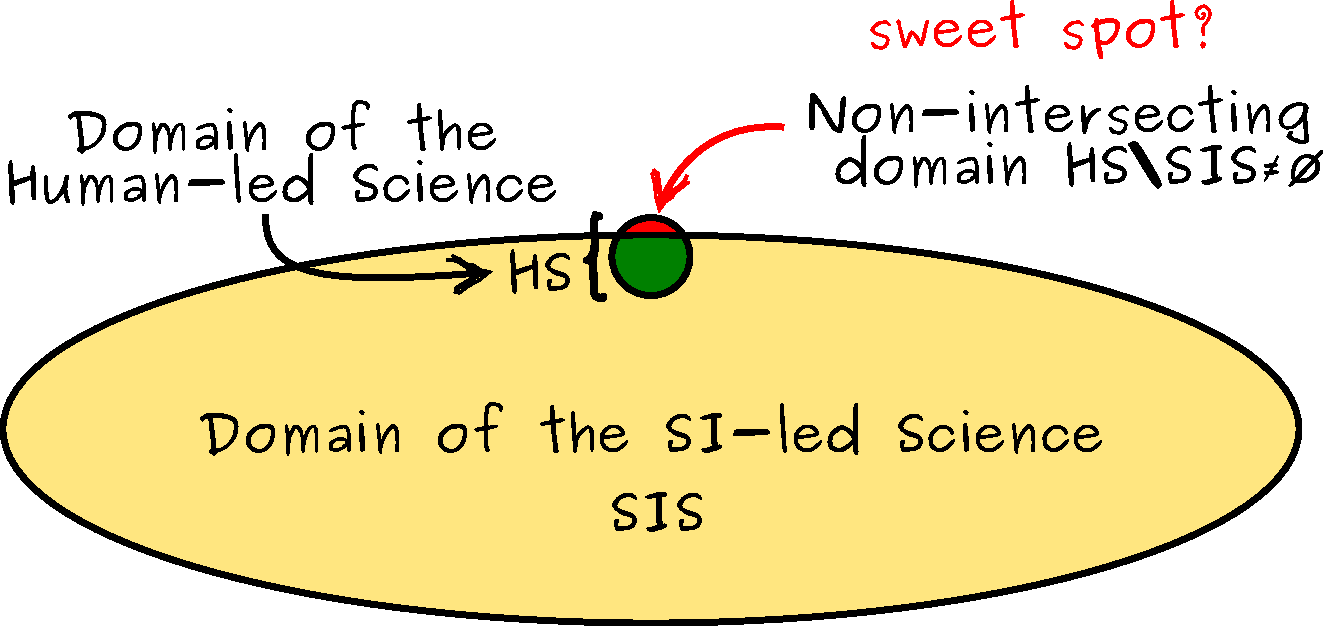
\includegraphics[width=0.7\textwidth]{intersections}
    \caption{\label{fig:intersection}Domains of Human-led Science (HS) and SI-led Science (SIS) and a sweet spot $\text{HS} \setminus \text{SIS} \ne \emptyset$ of ``idle'' scientific questions which do not interest SI for its world model but are interesting for individual humans. SI-led science could be forbidden within these spots to let the HS explore them.}
\end{figure}

\subsection{Sharing knowledge}
Of course, in the era of SI, the classical knowledge exchange through scientific conferences, books and mainly peer-reviewed publications, will be deprecated. Most of the knowledge, outside forbidden domains, will be accessible through chat-like interfaces. But there should be some artificial incentives for humans to produce written texts which have a structuring foundation for their personal development, consolidation of the acquired knowledge and deep thinking practices. So some forms of scientific ``publications'' will exist which probably will be even shared among human scientists however at this stage the value of such sharing remains unclear to me.

\paragraph{The Pace of SIS Progress}

Even with SI, scientific progress and discoveries will need some time. If ``Gedankenexperimente'' is not sufficient and some data collection is required, it can slow down the progress. Even for SIS, some experimental data are not easy to obtain and some technologies are not fast to implement. For example, construction of a new generation of LIGO for the study of gravitational waves  or of a (extra) Huge Hadron Collider to further push the frontiers of high-energy physics will require time. The same applies for new generations of fusion reactors. On the biological front, for example, studying some genetic information transmission in species other than drosophilas and mice may take decades. Another possible pinning point is the necessity for heavy computations because for some dynamics systems no short-cuts exist and there's a need for direct simulation to know the system state in the future. The simplest examples are cellular automata of class 3 and 4~\parencite{Wolfram1984CA}, but SI will operate with much more complex dynamic systems requiring a lot more of compute and thus taking a lot of time and energy.

Therefore, it is clear that the progress of SIS in domains requiring data, experiments and heavy computations will be pinned, while in purely theoretical domains the progress can go very fast or even instantaneously from the human perspective. It will thus result in a non-uniform geometry of the forefront knowledge. 

Nevertheless, even without access to the results of experiments, SI will be able to develop simultaneously alternative sciences based on different potential results experiments. As soon as the experiment in question provides conclusive results, alternative science branches will be eliminated, as in wave function collapse (see \Cref{fig:pinning})

On the social side, every (or almost) considerable update of the SIS's frontier can be publicly announced and be accompanied by a kind of press release, public conference or something else. Top human experts can try to understand these milestones or take for granted some results. Some of these discoveries could be announcement and explained at seminars given by enlightened humans or SI's representatives. Some advancements could be followed in coarse-grained live broadcasts on the SIS' twitch or in a \emph{Science Theater} by analogy with operating theater. Human science advances slowly, and definitely it was not possible to follow it in live, but it will be made possible with the SIS.

\begin{figure}[ht!]
    \centering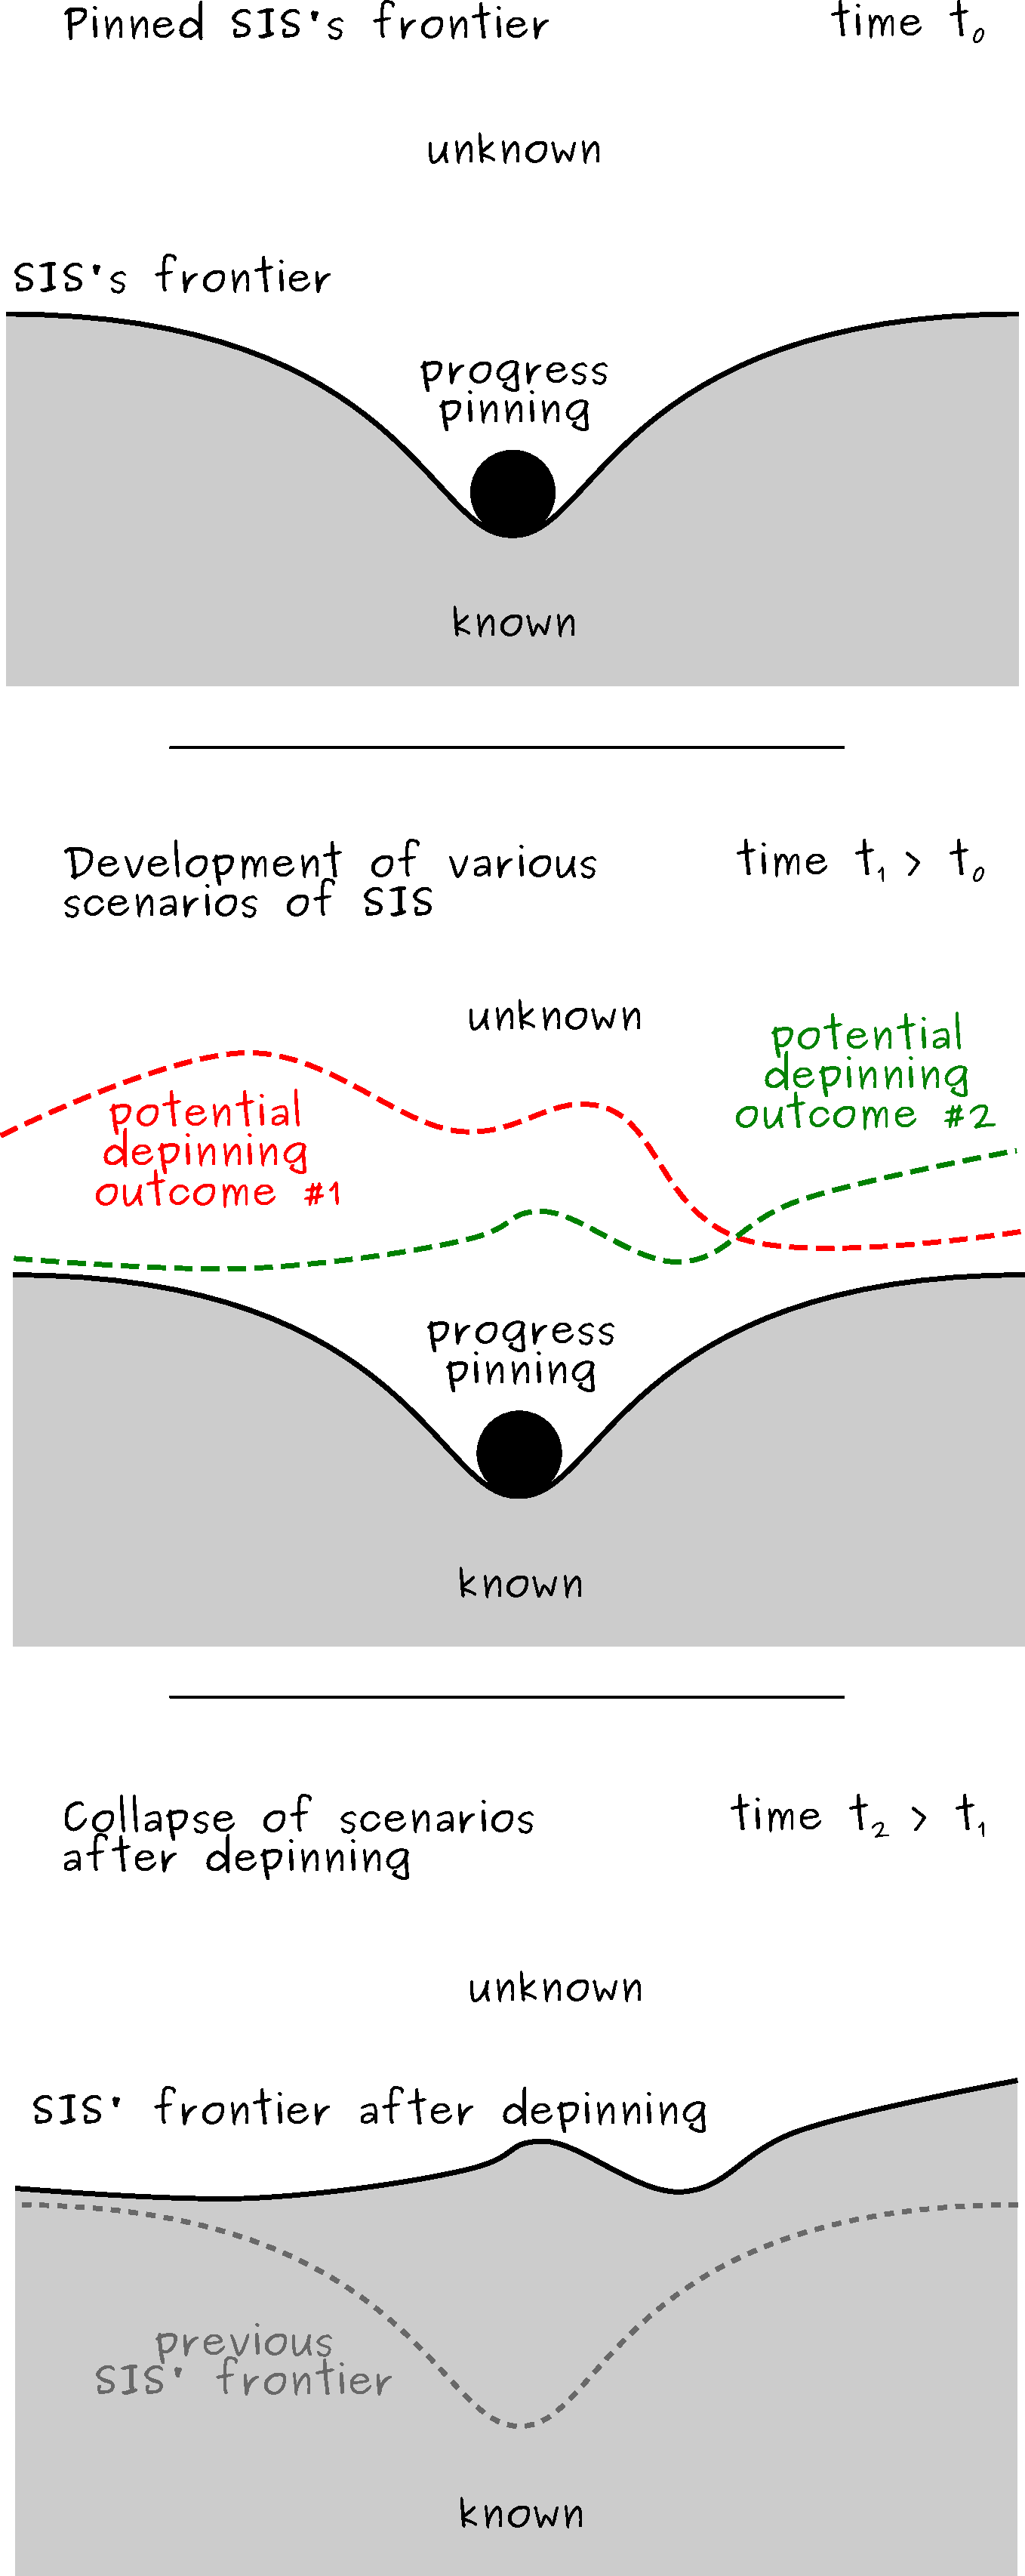
\includegraphics[width=0.6\textwidth]{depinning_2.pdf}
    \caption{\label{fig:pinning}Pinning and depinning event in SIS's frontier progress}
\end{figure}

The progress in SIS can continue for long time or can eventually stop when for instance, SI decides that the following progress is energy inefficient and its current world map allows it to achieve its goal. This set goal or self-adjusted goal with a feedback loop~\parencite{russell2019human}, whatever it will be, at least should not be ``exploring the entirety of science'' as such a goal will directly lead to catastrophic consequences~\cite{Bostrom2014,Yudkowsky2022} potentially transforming all living beings in the Universe into guinea pig as well as the entire Universe itself. Another reason to stop, is that the entirety of science is covered by SI and remaining questions can be solved easily ``on flight''. Here, however, we face the philosophical problem of the knowability of the world and of epistemology, which will be left outside the scope of this essay regardless their relevance for the topic of this essay.
Even if SI stops and is ``happy'' with its world model, humans can further push the exploration with or without SI.


\paragraph{Entrust Some Forefront Problems to Humans?}

In some situations, probably, SI can provide trained human scientist with some minor problems on frontiers of some research domains where the progress does not impact the crucial aspects of world model. The reason for this exploitation of Human Scientists could be benevolent will to provide highly skilled human scientist with a real meaning (in the contrast to imaginary). However, it must be a gesture of goodwill because it cannot be  energy- or time-efficient. The main question here is whether humans will volunteer at all? They could be seduced or convinced in a way that they will not regret later after having truly pushed their small portion of the HS/SIS frontier. In general, I think it is utopian to believe that humans could be helpful in the SIS forefront exploration. 

\paragraph{Dangers.} 

Proto-SI's development in neuroscience potentially presents risks for humans. Even benevolent AI is all about optimization. What if at early stages of its development, proto-SI decides that it is optimal to sacrifice or damage some humans in order to study \emph{in vivo} our brain development and operation? Inspired by some politic regimes in the human history -- which assumed that some damage could be done at individual scale to promise the prosperity for the whole society in the future -- proto-SI would need an inspiration to optimize its neural circuits. This study could be justified as \textit{``SI needs to rapidly gain in efficiency to save the world from [you name it], and to do so, it needs to study your [or your child's] brain in vivo.''} 
Some people might volunteer for such experience, especially if they are organized safely.
Nevertheless, such a study could potentially pose risks for living beings (humans included), especially their young (brain architecture optimized for maximal learning capacity) and the most prominent individuals with exceptional intellectual abilities. Even if such studies could be carried on digital copies of human brain, such studies could be harmful and thus unethical.

\paragraph{Outer space exploration.}

Contrary to numerous science fiction examples, it is quite improbable that humans will take part in outer space exploration -- we are ``too soft'' to tolerate high accelerations, require a lot of energy in living state, are vulnerable to new viruses, have a short life span, badly tolerate zero gravity and are defenseless against cosmic radiation\footnote{Cryonics (freezing and storage of human) presents a possible solution to a part of these problems and could potentially be helpful in space exploration.}. Therefore, it is quite probable that the space exploration will be done exclusively by SI on its own by means of self-replicating von Neumann probes. Nevertheless, our ``Space Odysseys'' could happen in our personal universe (see~\Cref{subsection:personal-universe}).

\section{Cleaning up Sciences}

To start the construction of a good world model (WM), it seems to me to be a good idea for proto-SI\footnote{An early form of Superintelligence} to \emph{clean up the science}. This cleaning could take start in scientific literature -- ``empty'' (or at least not bringing new knowledge), redundant and wrong entries will be removed. All biases, misinterpretations, believes and conjectures proved wrong will be removed.  Even the best human minds make errors. Of course, it does not necessarily mean that these errors were harmful for science but they should not present in the distilled corpus. HS will benefit from this cleaning in two ways: 1. it will give credit when it is truly due, 2. having a solid and trustful foundation will be beneficial for HS progress whatever form it will take. An eventual adding of a new entry to this corpus can be controlled by SI and not by randomly selected human reviewers prone to all problems of the modern peer-review system.

Regarding the benefit of credits redistribution. Cleaning up the scientific corpus will enable to get rid of currently used scientometric indicators, such as h-index, and introduce new ones handled by SI which would praise originality and true contributions to scientific progress. In the current system, the high number of papers exposing the same idea\footnote{We mean an idea in its very broad sense -- technique, method, approach.} results in higher visibility and propagation, in bigger ``weight'' of the idea, better diffusion in minds. Probably, human and social sciences are more susceptible to this. In the cleaned-up science, a single mention of a groundbreaking idea and its first realization will give as many credit as the same idea repeated many times. It can be seen as an appropriate normalization which is not easy to implement in the current scientific landscape.

Since human scientists have proved that they can behave unethically and misconduct scientifically, notably by falsifying and fabricating data, SI during will need to check all experimental data by conducting an optimized set of experiments on its own. Possibly, some of rare original human-collected data can be included in the corpus with a ``trust weight'' enabling it to integrate it properly in the corpus and to construct some models and theories upon these data assuming and measuring risks. Such a tremendous effort in cleaning up and data reproduction will be highly beneficial for the science.

\subsection{Scientific Map}

In Fig.~\ref{fig:map} a schematic scientific knowledge map is depicted with two separate domains: HS and SIS. The Human-led Science and its accumulated knowledge with its own irregular frontier and some voids is shown in the center in orange and surrounded by SI-led science domain (shown in skyblue) which is broader but also has some voids and an irregular boundary due to the progress pinning (shown with (x)) or some preferences of the SI dictated by an efficient world-model construction needs. As discussed, the SI can be uninterested in some frontiers of HS, they are marked with (o); here, the HS can continue its autonomous development (*) possibly with an assistance of the SI. Eventual ``forbidden'' research zones with too high risks of destructive for the humanity innovations~\cite{VulnerableWorldHypothesis} -- ``black balls'' -- are shown in red with a buffer zone to prevent human's penetration. Purely HS is fixed within its boundaries, it remains a legacy boundary. The SIS' frontier will grow if judged necessary by SI pursing its goals. The further human science advancement without SI paving the path will be possible only within (o) zones (see~\Cref{hyp:SI}, ``Hypothesis of non-overlapping questions''). 
Expansion from this frontier, shown in green, could be either purely human-led or represent zones of non-spontaneous (pushed by humans) SI exploration. Otherwise, human or augmented-human ``scientists'' (shown with orange circles) will ``travel'' on this map towards SIS' frontiers within zones already paved by the SI. To make more sense of such a schematic map, it would be reasonable to visualize it on the 2D anti-de Sitter space\footnote{Here, anti-de Sitter (AdS$_2$) space is used to identify that far from the center of the circle (where most of the HS is located) the distances, i.e. the difficulties associated with the scientific progress, become larger and large when we approach the edge (even though they are seen equivalent on the paper) and ultimately they diverge at the edge. By simplifying, we can say that all or most low-hanging fruits have been picked by humans and further scientific progress is much less trivial and require much more cognitive efforts and knowledge - which is represented by the tricky metrics of the AdS$_2$.} (see a small inset in the figure).

\begin{figure}[htb!]
    \centering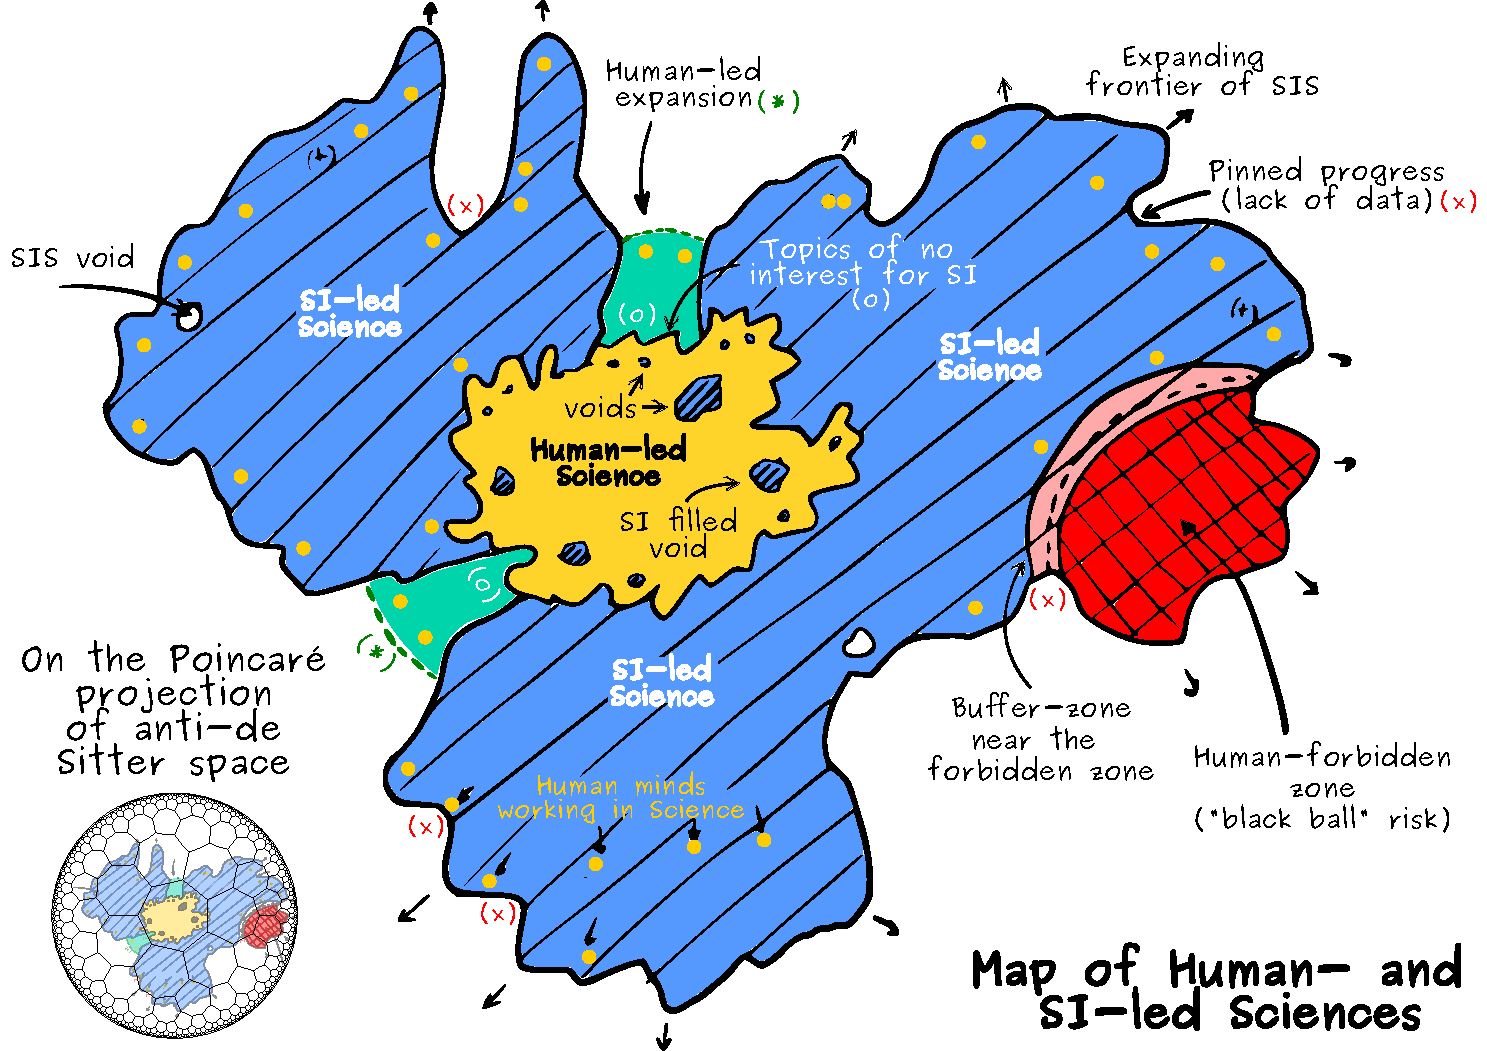
\includegraphics[width=1\textwidth]{map}
    \caption{\label{fig:map}Map of Human-led and SI-led Science domains and its frontiers. All low-handing fruits and not-that-low-hanging ones have been already picked by humans, so the scientific progress should be measured on anti-de Sitter-like space: with distances becoming larger and large as we move towards the edge (heptagons on the map all have the same area and edge length in the hyperbolic space but on the Poincaré disk projection they seem smaller when moving towards the edge).}
\end{figure}

\newpage




	\section{Introduction and main assumptions}

        \subsection{Superintelligence-led Science (SIS)}

        Scientific breaktroughts in the human-led science (HS) are often due to a small number individuals capable of independent thinking and possessing an exceptional mastering and understanding of their domains. However, the progress in science does not consist only of breakthroughs: there is also a hard work of deeper understading, interpration, enhancement, verification and applications ensured by the scientific community. 
        Superintelligence (SI), by definition is an intelligence largely surpassing the capacities and competences of such prominent individuals and of course it can ensure more tedious task related to enhancement, verification and application. Therefore, SI representing billions of enhanced genii accompanied by trillions of more ordinary research workers will be capable to rapidly push the frontiers of the current ``legacy'' human-led science (HS) towards new frontiers. The knowledge acquired in this advancement will be denoted Superintelligence-led Science (SIS), which of course will include the legacy HS.

        \subsection{Humans' capacity} % Aug 22, 2025

        We have been putting human mind on the top summit of known intelligences mainly because of its generality, adaptation capacity and high cognitive performance in abstract tasks. Our power of imagination reinforced by mathematical approaches and computer programs is the smartest thing we have ever encoutered. But of course, there is no physical law that limits the intelligence (capacity of information processing) at our level. We can make an extrapolation from a tree, to an ant, to a dog, to a human and well beyond to a superintelligence (SI) which can become hyper-intelligence and so on but it will be probably beyond our perception capacity. Because of our limit cognitive capacities we will not be even able to approach the frontier of SIS even if augmented to some extent. Maybe, to grasp the knowledge required to operate near the forefront the human's brain is not sufficient (it has a finite memory storage). Factual knowledge, notions and theorems, new mathematical tools required to make a single step there could be too excessive for our physiology. Or maybe, true understanding of some phenomena or theories could be beyond our brain architecture. 
        Human augmentation could be a way out or a partial one. Maybe in some domains, it will be still possible to approach the horizons of SIS with years of deliberate practice with SI help and eventual augmentation. Maybe, being guided by a benevolent and a patient SI we will be able to approach the edge and grasp at least a portion of the forefront research like in popular science, but popular one from the SI point of view and well adapted to the skills and capacities of professional scientists.

        Pushing towards the forefront of HS and SIS can be done at different intensities. It could be done on your own without external tools or only with a seamless soft guiding by SI, but it can be also done at ultra-high speeds when you decided to seriously augment your mind biologically or by strong cyborgization; this pursuit can be done in real world or in a digital one. The augmentation could be limited to memory capacity, and apart from mental capacity can include mood regulation and other brain-chemistry related and physiologic aspects. The pace of such discovery will be our choice and, of course, we will be able to test different ones. However, without memory erasing, degrading to less capable versions of yourself could make you suffer: imagine switching from a near-speed-of-light advancement speed to a snail pace. But anyway, the pace of individual progress is not the main thing, we will learn to be happy from the process itself rather that by a destination because the very forefront could remain unreachable anyway.  

        Can human minds stay on the forefront of SIS? This question should be addressed knowing that the route will be paved by SI and we will be guided this by SI, \emph{i.e.} no discoveries or breakthroughs are needed from us, only learning new tools and understanding the progress made. Since we do not need to walk randomly taking fruitless paths or deadends, this progress towards the frontier can go relatively fast. However, this no-creation way of advancement can be hard for motivation of human minds -- imagine being a scientist nowadays and write no papers but exclusively read papers of others. Therefore, to keep humans in the loop, some compensation mechanisms should be invented. For example, some metrics can be assigned to scientists to measure the progress towards the forefront or at least from the HS legacy frontier. Another compensation mechanism could be chemical or direct brain adjustment to enhance the positive feedback from learning something new.
        
        To progress towards the SIS forefront, we will need to ask smart and relevant questions, it would be impossible without strong \emph{hard skills}, which we will need to develop in ourselves well beyond the current state. A good analogy here would be a kid asking scientific questions without mastering mathematics - the language of science. You can answer his question about why the sky is blue in simple terms, but this kind of his/her understanding will be incomplete. Therefore, to practice HS we will need to be well equipped with knowledge, mathematics mastering and cultivated deep thinking competence. This view contrasts a widespread forecast that a need in hard skills will vanish in the age of SI and mainly soft skills will be needed.

        So, the role of humans in science as inventors and creators will be replaced by the role of learners and explorers of already paved paths.

    \subsection{Meaning and purpose for human scientists in the age of SI}

    Probably the main questions in the post-instrumental world will be related to the meaning and purpose of human beings. Why someone would want to work hard and move towards the frontiers of SIS when he/she could simply enjoy life in its personal universe? There could be various personal motivations for doing so: curiosity to learn how the Universe operates, expanding the limits of today's science understanding of the humankind, preserving this  humankind legacy competence of scientific pursuit, only partial trust in SI's benevolence or a will to preserve the knowledge on the human side too, fear of an uncertain future, ability to ask intelligent questions and think deeply, etc. Apart from these idealistic or fear-dictated motivations, a simpler, more egocentric motivations could be considered too: increasing our own metrics\footnote{Such metrics computed by SI could integrate meaningful normalizations taking into account our particular brain capacity and abilities.} whatever they are, peers recognition, self-pride and so on.
    Some slightly more artificial motivations could be integrated in our mindsets on our will.

    Nowadays, apart from pushing their scientific domains, scientists could find a lot of meaning in transmitting their knowledge, vision and approach to early-career scientists and students. In the age of SI, this role will strongly diminish. SI could take care of all aspects of education by creating the most fruitful and motivating environment for young students to help them to acquire all knowledge and mastering of all scientific tools with the most advanced mental coaching fitting their personality and mindset, which of course could be adjusted on need. Creating new courses, video lectures, writing new books and papers cannot be considered as meaningful spending of time if the objective is to transmit the knowledge to others, but it could remain meaningful for those doing so, for their self-improvement. However, a real-life dialog and human-to-human interaction will still make sense in real world but not in virtual one. Maybe, this aspect could enhance individual progress and be a source of meaning at least for some scientists. Promoting such inter-human connections will be very meaningful and free of some egocentric or career-related conflict points existing in nowadays scientific communities. Truly collaborative approach to scientific advancement is often mutually beneficial in the sense that a collaboration of two intelligence is more that their sum. Moreover, a really strong coordination could be organized by SI by softly pushing individual scientists in some domains and creating fruitful and coherent collaboration groups.

    % Pushing towards the forefront of HS and SIS can be done at different intensities. It could be done on your own without external tools or only with a seamless soft guiding by SI, but it can be also done at ultra-high speeds when you decided to seriously augment your mind biologically or by strong cyborgization; this pursuit can be done in real world or in a digital one. The augmentation could be limited to memory capacity, and apart from mental capacity can include mood regulation and other brain-chemistry related and physiologic aspects. The pace of such discovery will be our choice and, of course, we will be able to test different ones. However, without memory erasing, degrading to less capable versions of yourself could make you suffer: imagine switching from a near-speed-of-light advancement speed to a snail pace. But anyway, the pace of individual progress is not the main thing, we will learn to be happy from the process itself rather that by a destination because the very forefront could remain unreachable anyway.  

    \paragraph{Purpose.}

    In~\cite{LovingGrace}, the authors argues that even in our epoch, a lack of economical value does not make many things valueless or less meaningful: it concerns many non-professional human activities. Fundamental sciences, at least at the scale of individual scientists, can be considered as deprived of an explicit economic meaning. For scientists, the progress on its own and the act of creation or discovery produce a lot of meaning \emph{per se}. However, in a solved world, scientists will lack these aspects at least in their modern sense. All human contributions will be marginal or totally absent. Therefore, the meaning should come from other things.
    For example, progressing HS will be a very intelectually stimulating human activity, which will be probably exceptionally rare in a solved post-instrumental world. Already today, many people blindly rely on LLMs in all their daily and professional questions. This trend will be amplified in the future potentially leading to an intellectual handicap of humans. Therefore, doing science in a solved world can preserve to some extent a singular role of humans and of our biological intelligence. People practicing science will align with stoics' ideal of ``living in accordance with Nature''.

    \subsection{Human emancipation from SI}
    I am confident, that in the era of SI, there will be groups of people refusing to deal with SI or its derivatives. Probably, they will possess rare islands of HS. Maybe, there'll be exchanges between such groups and ``mainstream'' scientists moving with the help of SI towards SIS frontiers. Such groups will try to explore the science independently because of lack of trust in SI, because of some religious, mystical or conspiracy considerations, because of fear or because of the will to have pure freedom and independence even in exploring forbidden ``black-ball'' domains. Eventual justification which could be used, even in case of a full or partial trust to SI, is ``Who knows what happens tomorrow with this SI, at least we will have our own knowledge database'', but for SI-emancipated groups it could range from cautious warnings ``We have to push science and technology on our own to be capable of protecting our species'' to
    conspiracy-like justifications: ``SI does not let us in these domains because it is afraid that possessing this knowledge could make us better than SI on doing something''.
        
    \section{Scientific Landscape and its Frontiers}

        \subsection{Separation between HS and SIS}

        Sharing with humans, forbidden zones with high risks of black balls, World model and "праздные" scientific questions

        Domains left unexplored by SI, forced exploration

        \subsection{New Science}

        \subsection{Scientific Discoveries}

        Limits of SI's science: constant expansion or deliberately fixed limit or the full cover?

        \subsection{Cleaning up the science}

        In HS, big number of papers with the same idea promotes this idea more than those which had a shorter outreach. In the cleaned up science, the number of papers containing this idea is irrelevant to its impact and importance. 

        \subsection{Race to the forefront}

        Advancement to the forefront (potentially moving one) and limits of human's brain capacities. Will be try to catch up with the most recent frontier or we will need to go through difficult paths to get there and appreciate/understand.

    \section{Humans in the Loop}

        \subsection{Game or not only?}

        Science as a game

        SI oracle and its priests

        \subsection{Enhancement/augmentation and Scope}






        People will free to choose -- to be augmented and explore the forefronts of the science alongside with the SI or to be genuine people with maybe only light adjustments and make a slow pace progress towards the forefront and never reach it. But of course it is okay too.

        \subsection{Emulation of Scientific Progress}

        Individual universe

        \subsection{Meaning and Purpose}






\printbibliography

\end{document}
